\chapter{Thermodynamique (sup)}

\newpage

\section{Chute d'une masse sur un piston $\bullet\bullet\bullet\circ$}

On considère un gaz parfait, de coefficient $\gamma$, à la température $T_0$, contenu dans un cylindre de section $S$ surmonté d'un piston, situé à une hauteur $a$ par rapport au fond du dispositif. Le piston, de masse négligeable, peut coulisser sans frottement et toutes les parois sont isolées thermiquement de l'extérieur, où la pression et la température sont respectivement $P_0$ et $T_0$. Le champ de gravitation est modélisé par la constante d'accélération $g$.

\begin{figure}[h!]
\centering
  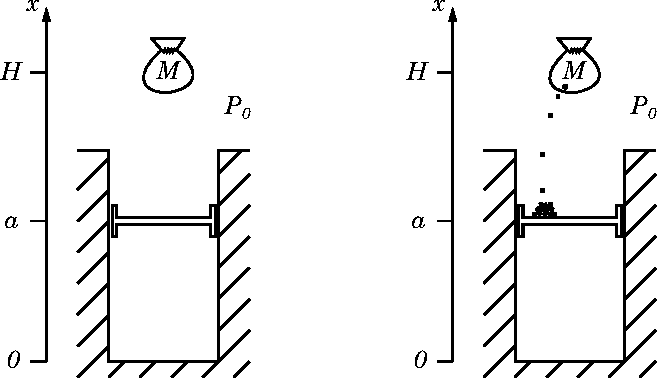
\includegraphics[width=0.8\textwidth]{thermo_sable.pdf}
\end{figure}

Au dessus du piston, à une altitude $H$ (repérée par rapport au fond du cylindre), se trouve un sac de sable de masse totale $M$. On souhaite étudier dans un premier temps le cas où le sac de sable tombe d'un bloc sur le piston (shcéma de gauche), et puis la situation où la totalité du sable se déverse grain par grain sur le piston (schéma de droite).

\begin{enumerate}

\item Dans ce cas-là, on considère que le sac de sable tombe d'un bloc sur le piston.

\begin{enumerate}

\item A quel type de transformation a t-on affaire dans ce cas-là ? Décrire qualitativement ce qu'il se passe.

\item Calculer la hauteur $x$ finale du piston après le retour à l'équilibre.

\item En déduire qu'il existe une hauteur $H_c$ critique à laquelle le piston remonte, à la suite du choc, à la même hauteur initiale $a$. Donner son expression et décrire qualitativement ce qu'il se passe si $H<H_c$ ou $H>H_c$.

\end{enumerate}

\item On suppose désormais que le sac est percé d'un petit trou, laissant sortir les grains de sables les uns après les autres.

\begin{enumerate}

\item A quel type de transformation a t-on affaire dans ce cas-là ? Quelle différence avec le cas précédent ?

\item Quel est le déplacement $dx$ du piston après la chute d'un grain de sable de masse $dm$ ?

\item Calculer la hauteur $x$ finale du piston une fois tout le sable tombé dessus. Comparer cette expression avec celle trouvée précedemment et commenter.

\end{enumerate}

\end{enumerate}

\newpage

\begin{correction}

\begin{enumerate}

\item

\begin{enumerate}

\item C'est une transformation brutale. Les paramètres du gaz dans le cylindre ne sont pas définis durant cette transformation ; on ne peut considérer que les états initiaux et finaux. Il va y avoir échauffement du gaz car l'énergie potentielle de la masse sera transférée sous forme de chaleur, ainsi que sous le travail des forces de pression extérieur.

\item Etat inital du gaz : $(P,T,V) =(P_0,T_0,aS)$. Etat final : $(P,T,V) =(P_f,T_f,xS)$ (3 inconnues, il faut donc trois équations). L'équilibre mécanique implique : $P_f=P_0+Mg/S$. L'équation des gaz parfait et le premier principe permettent d'obtenir deux autres équations indépendantes. 

Le premier principe appliqué au système {masse $M$ ; gaz} donne :
\begin{align*}
	\Delta U + \Delta E_p &= W \\
	\frac{nR}{\gamma-1}(T_f-T_0)+Mg(x-H)=&-P_0S(x-a)
\end{align*}
On précise que la variation d'énergie interne de la masse $M$ et d'énergie potentielle du gaz sont négligeable. D'autre part, $Q=0$ car pas d'échange thermique avec l'extérieur. Enfin, le travail de pression se fait à \textbf{pression extérieure constante} $P_0$ donc $W=-P_0S(x-a)$. En utilisant la loi des GP, on trouve :
\begin{align*}
	x(P_0S+Mg)=\frac{\gamma-1}{\gamma}MgH+P_0Sa
\end{align*}

\item On a retour à la hauteur initiale si $x=A$, alors $H_c=\frac{\gamma}{\gamma-1}a$. Si $H<H_c$, le piston s'enfonce plus bas que $a$ : l'énergie du choc ne dégage pas assez d'énergie thermique pour soulever le poids du sac. Si $H>H_c$, le piston s'élève par rapport à $a$.

\end{enumerate}

\item

\begin{enumerate}

\item C'est une transformation que l'on peut considérer comme inifiniment lente, donc réversible : chaque grain de sable faisant que très légèrement bouger le piston. Les paramètres du gaz sont constamment définis.

\item On utilise le même raisonnement que précédemment. On considère une transformation $(T,P,V)\longrightarrow(T+dT,P+dP,V+dV$ après la chute d'un grain de sable de masse $dm$. On a : $dP=gdm/S$ (équilibre des pressions) et $dV=Sdx$.
Premier principe :
\begin{align*}
	\frac{nRdT}{\gamma-1}+dmg(x-H)=&-P_0Sdx
\end{align*}
Or la loi des gaz parfaits donne :
\begin{align*}
& (P+dP)(V+dV)=nr(T+dT) \\
\Rightarrow \quad & P_0Sdx+dmgx=nRdT
\end{align*}
(ce qui revient différencier cette loi). 
On a donc :
\begin{align*}
P_0Sdx=dmg\left(\frac{\gamma-1}{\gamma}H-x \right) 
\end{align*}
\textit{NB} : on retrouve bien le résultat de la question précédente, avec $dx$ positif ou négatif si $H$ supérieur ou inférieur à $H_c$.

\item Il faut intégrer la relation précédente. En posant la variable intermédiaire $u=\frac{\gamma}{\gamma-1}\frac{x}{H}$, on trouve :
\begin{align*}
 \int_{\frac{\gamma}{\gamma-1}\frac{a}{H}}^{\frac{\gamma}{\gamma-1}\frac{x}{H}}\frac{du}{1-u}=\frac{Mg}{P_0S}
\end{align*}
On trouve alors :
\begin{align*}
x=\frac{\gamma-1}{\gamma}H(1-e^{-\frac{Mg}{P_0S}})+ae^{-\frac{Mg}{P_0S}}
\end{align*}

\end{enumerate}

\end{enumerate}

\end{correction}

\newpage	

\section{Entropie d'une chute libre $\bullet\bullet\bullet\circ$}

On considère un gaz parfait, de coefficient $\gamma$, à la température $T_0$, contenu dans un cylindre de section $S$ surmonté d'un piston, situé à une hauteur $a$ par rapport au fond du dispositif. Le piston, de masse négligeable, peut coulisser sans frottement et toutes les parois sont isolées thermiquement de l'extérieur, où la pression et la température sont respectivement $P_0$ et $T_0$. Le champ de gravitation est modélisé par la constante d'accélération $g$.

\begin{figure}[h!]
\centering
  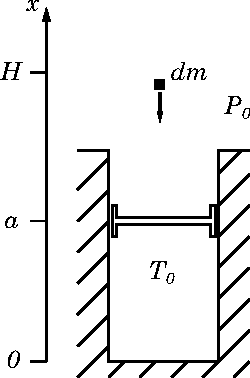
\includegraphics[width=0.3\textwidth]{thermo_sable_bis.pdf}
\end{figure}

On fait tomber un grain de sable de masse $dm$ sur le cylindre, d'une hauteur $H$.

\begin{enumerate}

\item A quel type de transformation a t-on affaire ?

\item Quel est le déplacement $dx$ du piston après la chute d'un grain de sable de masse $dm$ ?

\item En déduire la variation d'entropie du gaz $dS_g$ lors de cette transformation. On rappelle que, pour un gaz parfait de $n$ moles, la variation d'entropie lors d'une transformation élémentaire s'écrit :
\begin{align*}
	dS=\frac{nR}{\gamma-1}\left(\frac{dP}{P}+\gamma\frac{dV}{V} \right) 
\end{align*}

\item En déduire que l'entropie créée par la chute d'une masse $M$ d'une hauteur $H$ à la température $T_0$ s'écrit :
\begin{align*}
	s_c=\frac{MgH}{T_0}
\end{align*} 

\end{enumerate}

\newpage

\begin{correction}

\begin{enumerate}

\item Cf exercice précédent. C'est une transformation que l'on peut considérer comme inifiniment lente, donc réversible : chaque grain de sable faisant que très légèrement bouger le piston. Les paramètres du gaz sont constamment définis.

\item Cf exercice précédent :
\begin{align*}
P_0Sdx=dmg\left(\frac{\gamma-1}{\gamma}H-x \right) 
\end{align*}

\item Avec la formule donnée :
\begin{align*}
	dS_g&=\frac{nR}{\gamma-1}\left(\frac{dP}{P}+\gamma\frac{dV}{V} \right) \\
	&=\frac{nR}{\gamma-1}\left(\frac{dmg}{SP_0}+\gamma\frac{dx}{x} \right) \\
	&=dm\frac{nRg}{(SP_0}\left(\frac{H}{x}-1 \right)
\end{align*}
Or, $nR/P_0=V_0/T_0=Sx/T_0$, donc :
\begin{align*}
	dS_g&=dm\frac{g}{T_0}(x-H)
\end{align*}
Pour une masse $M$ au lieu de $dm$, on obtient le résultat escompté. 

\item La variation d'entropie du système {gaz ; $M$} s'écrit :
\begin{align*}
	dS = dS_g+dS_M=\delta s_c + \delta s_e
\end{align*}
Comme il n'y a pas de transferts thermiques, $\delta s_e=0$. D'autre part, l'entropie de la masse $M$ ne change pas car il reste à tempréature constante. Lors de cette transofmration on a donc :
\begin{align*}
	s_c=\frac{MgH}{T_0}
\end{align*} 

\end{enumerate}

\end{correction}

\newpage

\section{Machine de Stirling $\bullet\bullet\circ\circ$}

On considère une machine thermodynamique, constituée d'un cylindre dans lequel coulisse un piston, qui effectue les transformations suivantes sur $n$ moles gaz parfait de coefficient $\gamma$ : 

\begin{itemize}
\item[$A \rightarrow B$ :] compression isotherme du volume $V_A$ au volume $V_B$, réversible, à la température $T_f$ (contact avec une source froide) ;
\item[$B \rightarrow C$ :] échauffement isochore ;
\item[$C \rightarrow D$ :] détente isotherme de $V_B$ à $V_A$, réversible à la température $T_c$ (contact avec une source chaude) ;
\item[$D \rightarrow A$] : refroidissement isochore.

\end{itemize}

Le cycle de Stirling a l'avantage de pouvoir être réalisable en pratique sur des dispositifs appelés \textit{moteurs de Stirling}, contrairement au cycle de Carnot, théorique.

\begin{enumerate}

	\item Décrire ce cycle dans un diagramme de Clapeyron $(P,V)$ et justifier qu'il est moteur.

	\item Déterminer, pour chaque transformation, $\Delta U$, $W$, et $Q$ en fonction de températures de la source chaude et de la source froide et du rapport de compression $a=V_A/V_B$.
	
	\item  Calculer son rendement $\eta$, et montrer qu'il est nécessairement inférieur au rendement de Carnot $\eta_C$.
	
	\item Avec un système appelé regénérateur, il est possible de stocker momentanément la chaleur évacuée de $D \rightarrow A$, pour la retransférer durant la transformation $B \rightarrow C$. Calculer le rendement $\eta'$ avec ce dispositif.
		
\end{enumerate}

\newpage

\begin{correction}

\begin{enumerate}

	\item Facile à représenter. Le cycle est moteur car il tourne dans le sens horaire donc l'intégrale $W=-\oint PdV<0$

	\item Pour le calcul du travail pour une transformation isotherme, on a :
		\begin{align*}
	W = -\int_i^f P\dif V &= nRT\ln\left(\frac{V_i}{V_f} \right) 
\end{align*}
	\begin{center}
\begin{tabular}{|p{2,5cm}|p{3cm}|p{3cm}|p{3cm}|}
\hline
Transformation & $\Delta U$ & $W$ & $Q$ \\
\hline
$A\rightarrow B$ & 0  & $nRT_f\ln a$  & $-nRT_f\ln a$  \\
\hline
$B\rightarrow C$ & $\frac{nR}{\gamma-1}(T_c-T_f)$ & 0 & $\frac{nR}{\gamma-1}(T_c-T_f)$  \\
\hline
$C\rightarrow D$ & 0  & $-nRT_c\ln a$ & $nRT_c\ln a$ \\
\hline
$D\rightarrow A$ & -$\frac{nR}{\gamma-1}(T_c-T_f)$ & 0 & -$\frac{nR}{\gamma-1}(T_c-T_f)$ \\
\hline
\end{tabular}
\end{center}
	
	\item  La chaleur apportée par souce chaude est $Q_c=Q_{C\rightarrow D}+Q_{B\rightarrow C}$. Le rendement $\eta$ est donc
	\begin{align*}
		\eta&=\frac{-W}{Q_c}=\frac{nR(T_c-T_f)\ln a}{\frac{nR}{\gamma-1}(T_c-T_f)+nRT_c\ln a} \\
		&=\frac{T_c-T_f}{T_c+\frac{T_c-T_f}{\ln(a)(\gamma-1)}}
	\end{align*}
	Or le rendement de Carnot est $\eta_C=\frac{T_c-T_f}{T_c}$ : ce dernier est supérieur car le dénominateur de la fraction est inférieur.
	
	\item Dans ce cas-là, le rendement devient :
	\begin{align*}
		\eta&=\frac{-W}{Q_c-Q_{B\rightarrow C}}=\frac{nR(T_c-T_f)\ln a}{nRT_c\ln a} \\
		&=\frac{T_c-T_f}{T_c} \\
		&=\eta_C
	\end{align*}	
		
\end{enumerate}

\end{correction}

\newpage

\section{Cycle de Beau de Rochas $\bullet\bullet\circ\circ$}

Les moteurs à essence équipant la plupart des véhicules terrestres sont des machines thermodynamiques généralement constitués de plusieurs cylindres, dans lequels un piston fait subir sur $n$ moles de gaz parfait le cycle suivant (dit de Beau de Rochas) :

\begin{itemize}

\item[$A \rightarrow B$ :] compression adiabatique, réversible du volume $V_A$ au volume $V_B$ : le mélange d'air frais et essence est comprimé ;
\item[$B \rightarrow C$ :] échauffement isochore en contact de la source chaude, en pratique il s'agit de la combustion très rapide de l'essence dégageant une chaleur $Q_c$ ;
\item[$C \rightarrow D$ :] détente adiabatique, réversible du volume $V_B$ au volume $V_C=V_A$ : les gaz de combustion "poussent" le cylindre en fournissant du travail ;
\item[$D \rightarrow A$ :] refroidissement isochore en contact de la source froide : les gaz issus de combustion sont évacués et remplacés par par un mélange d'air frais et d'essence. Le cycle reprend ensuite.

\end{itemize}

Ce cycle de fonctionnement a l'avantage de pouvoir faire varier la puissance du moteur très rapidement, car il est facile de contrôler la quantité de chaleur $Q_c$ apportée par la combustion de l'essence lors de la transformation $B \rightarrow C$. On souhaite montrer que cet avantage pratique se fait néanmoins au détriment du rendement $\eta$, qui est nécessairement inférieur au rendement de Carnot $\eta_C$.

\begin{enumerate}

	\item Décrire ce cycle dans un diagramme de Clapeyron $(P,V)$ et justifier qu'il est moteur.

	\item Déterminer, pour chaque transformation, $\Delta U$, $W$, et $Q$ en fonction de températures $T_A$, $T_B$, $T_C$ et $T_D$ atteintes aux moments $A$, $B$, $C$ et $D$.
	
	\item Exprimer les températures $T_B$, $T_C$ et $T_D$ à partir de $T_A=300$K, la température de l'air ambiant, et de $Q_c$, la chaleur dégagée par la combustion d'essence. Pour simplifier l'écriture, on pourra utiliser le taux de compression $a=V_A/V_B$.
	
	\item  Calculer son rendement $\eta$ en fonction de $a$ et $\gamma$, et montrer qu'il est nécessairement inférieur au rendement de Carnot $\eta_C$.
	
	%\item Calculer l'entropie crée $s_c$ sur un cycle. Commenter.
	
\end{enumerate}

\newpage

\begin{correction}

\begin{enumerate}

	\item Facile à représenter. Le cycle est moteur car il tourne dans le sens horaire donc l'intégrale $W=-\oint PdV<0$

	\item On peut proposer d'effectuer le calcul suivant pour le calcul du travail :
	\begin{align*}
	W = -\int_i^f P\dif V &= -cste\int_i^f \frac{\dif V}{V^{\gamma}}\\
	&=-cste\frac{V_f^{1-k}-V_i^{1-k}}{1-k}\\
	&=\frac{P_fV_f-P_iV_i}{\gamma-1}\\
	&= \frac{nR}{\gamma-1}(T_f-T_i)
\end{align*}
Appliquer le premier principe suffit aussi. On utilise le résultat précédent pour les transformations $A\rightarrow B$ et $D\rightarrow A$. Pour les transformations isochores, on calcule $\Delta U$ tout simplement pour l'échauffement d'un gaz.

\begin{center}
\begin{tabular}{|p{2,5cm}|p{3cm}|p{3cm}|p{3cm}|}
\hline
Transformation & $\Delta U$ & $W$ & $Q$ \\
\hline
$A\rightarrow B$ & $\frac{nR}{\gamma-1}(T_B-T_A)$  & $\frac{nR}{\gamma-1}(T_B-T_A)$  & 0  \\
\hline
$B\rightarrow C$ & $\frac{nR}{\gamma-1}(T_C-T_B)$ & 0 & $Q_c=\frac{nR}{\gamma-1}(T_C-T_B)$  \\
\hline
$C\rightarrow D$ & $\frac{nR}{\gamma-1}(T_D-T_C)$  & $\frac{nR}{\gamma-1}(T_D-T_C)$ & 0 \\
\hline
$D\rightarrow A$ & $\frac{nR}{\gamma-1}(T_A-T_D)$ & 0 & $Q_f=\frac{nR}{\gamma-1}(T_A-T_D)$ \\
\hline
\end{tabular}
\end{center}

\item On détermine la température à chaque transformation :
\begin{itemize}
	\item[$A\rightarrow B$ :] $T_B=a^{\gamma-1}T_A$ car compression adabatique en utilisant $TV^{\gamma-1}=cste$.
	\item[$B\rightarrow C$ :] $T_C=\frac{nR}{\gamma-1}Q_c + T_B$, d'après le premier principe : on échauffe le gaz en lui apportant $Q_c$.
	\item[$C\rightarrow D$ :] $T_D=T_C/a^{\gamma-1}$ car compression adabatique.
\end{itemize}


 \item  Pour calculer le rendement, il faut expliciter la quantité de chaleur $Q_c$ issue de la source chaude : il s'agit de $Q_{AB}$, car on augmente la pression à volume constant, c'est-à-dire qu'on apporte de la chaleur. Ici, elle est apportée par l'explosion de l'essence. Le travail total sur un cycle, quant à lui, s'écrit :

\begin{align*}
	W &= -\frac{nR}{\gamma-1}(T_B-T_A+T_D-T_C)\\
	&=-\frac{nR}{\gamma-1}(T_D-T_A) + Q_c
\end{align*}
On a donc :
\begin{align*}
	T_D = \frac{\gamma-1}{a^{\gamma-1}nR}Q_c+T_f
\end{align*}

Donc $W=Q_c\left( 1-\frac{1}{a^{\gamma-1}}\right) $ et alors :
\begin{align*}
	\eta= 1-\frac{1}{a^{\gamma-1}}
\end{align*}

	Pour comparer avec le rendement de Carnot $\eta_C=1-T_f/T_c$, il faut expliciter les températures de la source chaude $T_c$ et froide $T_f$. La température de la source chaude est à priori $T_C$ car le gaz est au maximum de sa température en $C$. En effet, comme la transformation $C\longrightarrow D$ est réversible, elle est supposée très lente, donc on peut supposer que le gaz s'est thermalisé à la température de la source chaude en $C$. 
	
	A ce moment là :
	\begin{align*}
		\eta_C&=1-\frac{T_A}{T_C}\\
		&=1-\frac{T_A}{\frac{\gamma-1}{nR}Q_c+a^{\gamma-1}T_A}\\
		&=1-\frac{1}{\frac{\gamma-1}{nRT_A}Q_c+a^{\gamma-1}}\\
		&>1-\frac{1}{a^{\gamma-1}} = \eta
	\end{align*}

On retrouve bien le fait que le rendement de Carnot est supérieur.

\end{enumerate}

\end{correction}

\newpage

\section{Compression brutale $\bullet\bullet\circ\circ$}

On considère le dispositif ci-dessous : un piston pouvant coulisser librement dans un cylindre, tous deux ayant des parois adiabatiques. Une paroi interne sépare les espaces $A$ et $B$ est fixe et diatherme et est percée d'un trou fermé par une fenêtre amovible. La pression extérieure est $P_0=1$ bar. Initialement, le volume $A$ est rempli d'une mole de gaz parfait $\gamma=1,4$, avec une pression $P_0=1$ bar, une température $T_0=300$K, tandis que le volume $B$ est vide.

\begin{figure}[!h]
\centering
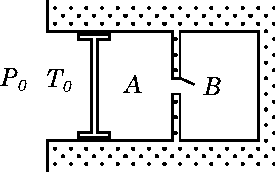
\includegraphics[width=0.5\linewidth]{thermo_pistonAB.pdf}
\end{figure}

\begin{enumerate}
\item On ouvre la fenêtre. Décrire qualitativement ce qu'il se passe suivant le volume de $A$ et $B$. En déduire l'existence d'un volume critique $V_C$ pour le volume $A$, que l'on ne demande pas de calculer ici.

\item On suppose $V_A<V_C$. Déterminez l'état final du gaz : on exprimera $V_f$ en fonction de $V_B$, $T_f$ en fonction de $T_0$ et $P_f$ en fonction de $P_0$. En déduire $V_C$.

\item Calculer la création d'entropie. Quelle est la cause de la création d'entropie ? On rappelle que lors d'une transformation $(P_i,T_i)\rightarrow  (P_f, T_f)$ sur $n$ moles de gaz parfait, on a :
\begin{align*}
	\Delta_i^f S=\frac{nR\gamma}{\gamma-1}\ln\left(\frac{T_f}{T_i} \right) - nR\ln\left(\frac{P_f}{P_i} \right)
\end{align*}

\item On suppose désormais que $V_A>V_C$. Quel est l'état final ?

\end{enumerate}

\newpage

\begin{correction}

\begin{enumerate}

\item Si $V_A\gg V_B$, alors tout le gaz se répartit dans $B$ sans que le piston ne touche la paroi interne. Inversement, si $V_A\ll V_B$, le piston va venir se coller contre la paroi interne et le gaz va intégralement dans $B$. Il y a donc une situation intermédiaire "limite" entre les deux où le piston va doucement se coller contre la paroi interne mais avec une équilibre des pressions.

\item Dans ce cas-là, le piston se colle contre la paroi : on a donc $V_f=V_B$. Il faut considérer le système {gaz+vide dans $B$} lorsqu'on applique le premier principe, avec donc $V_i=V_A+V_B$. Alors, comme la transformation est brutale, on a :
\begin{align*}
	\frac{nR}{\gamma-1}(T_f-T_0)&=W \\
	&=-P_0(V_f-V_i) \\
	&=-P_0V_A
\end{align*}
Avec la loi des gaz parfaits, appliqué sur le gaz contenu en $A$, on a $P_0V_A=nRT_0$, on trouve donc :  $T_f=\gamma T_0$ et $P_f=\gamma P_0V_A/V_B$.

Le volume critique est donc lorsqu'il y a équilibre des pressions : $P_0=P_f$, soit $V_A=V_C=V_B\gamma$.


\item Il n'y a pas d'échange de chaleur, donc $S_e=0$, alors $\Delta S=S_c$. On trouve :
\begin{align*}
	S_c=\Delta_i^f S=\frac{nR\gamma}{\gamma-1}\ln\left(\gamma \right) - nR\ln\left(\gamma\frac{V_A}{V_B} \right)
\end{align*}
L'entropie créée est bien positive, car on a $V_A<V_C$. Dans ce cas limite, on a $S_c=-nR\ln(\gamma-1)>0$.


\item On suppose désormais que $V_A>V_C$. Quel est l'état final ?

\end{enumerate}

\end{correction}

\newpage

\section{Compresseur à deux étages $\bullet\bullet\circ\circ$}

Pour de nombreux usages, on souhaite obtenir de l'air comprimé, c'est-à-dire de l'air à la température ambiante $T_0=300$K mais à une pression $P_1$ plus élevée que la pression atmosphérique $P_0=1$ bar, généralement $P_1=8$ bars. On notera $a=P_1/P_0$ le rapport de compression voulu.

\begin{enumerate}

\item On dispose dans un premier temps d'un cylindre muni d'un piston amenant $n$ moles de gaz parfait  (de coefficient $\gamma$) de l'état $(P_0, T_0)$ à l'état $(P_1, T_0)$ selon le chemin suivant :
\begin{itemize}

	\item[$A\rightarrow B$ :] compression adiabatique et réversible de $(P_0, T_0)$ à $(P_1, T_1)$ ;
	\item[$B\rightarrow C$ :] refroidissement isobare de $T_1$ à $T_0$.
	
\end{itemize}

Le refroidissement se fait avec une thermalisation avec l'atmosphère ambiant qui reste à $T_0$.

\begin{enumerate}

\item Représenter la transformation $(P_0, T_0)\rightarrow (P_1, T_0)$ dans un diagramme de Clapeyron.
\item Calculer le travail $W$ fourni par le piston durant cette transformation, en fonction de $P_0$, $V_0$ et de $a$. 
\item Calculer l'entropie créée $s_c$ et commenter.

\end{enumerate}

\item On souhaite diminuer le travail $W$ fourni pour comprimer le gaz. Pour cela, on comprime le gaz en deux temps, en ajoutant un étage de compression (en pratique un second cylindre à la suite du premier). La transformation du gaz est désormais :
\begin{itemize}

	\item[$A\rightarrow B$ :] compression adiabatique et réversible de $(P_0, T_0)$ à $(P_i, T_i)$ ;
	\item[$B\rightarrow C$ :] refroidissement isobare de $T_i$ à $T_0$ ;
	\item[$C\rightarrow D$ :] compression adiabatique et réversible de $(P_i, T_0)$ à $(P_1, T_1)$ ;
	\item[$D\rightarrow E$ :] refroidissement isobare de $T_1$ à $T_0$.
	
\end{itemize}

\begin{enumerate}

\item Représenter cette nouvelle transformation $(P_0, T_0)\rightarrow (P_1, T_0)$ dans un diagramme de Clapeyron.
\item Calculer le travail $W'$ fourni par le piston, en fonction de $P_0$, $V_0$, $P_1$ et $P_i$.
\item Comment doit-on choisir $P_i$ pour minimiser le travail fourni ? En déduire $W'$ pour cette valeur de $P_i$ et montrer que $W'<W$.
\item Calculer l'entropie créée $s_c'$. Comparer avec $s_c$ et commenter.

\end{enumerate}

\item Quelle serait la transformation pour que le travail fourni soit minimal ? Justifier à l'aide d'un diagramme de Clapeyron. Pourquoi est-ce difficilement réalisable en pratique ? Calculer alors l'entropie créée.

\end{enumerate}

On rappelle que lors d'une transformation $(P_i,T_i)\rightarrow  (P_f, T_f)$ sur $n$ moles de gaz parfait, on a :
\begin{align*}
	\Delta_i^f S=\frac{nR\gamma}{\gamma-1}\ln\left(\frac{T_f}{T_i} \right) - nR\ln\left(\frac{P_f}{P_i} \right)
\end{align*}

\newpage

\begin{correction}

\begin{enumerate}

\item

\begin{enumerate}

\item Pour le diagramme de Clapeyron, on peut passer du volume à la température avec la loi des gaz parfaits.

\centering
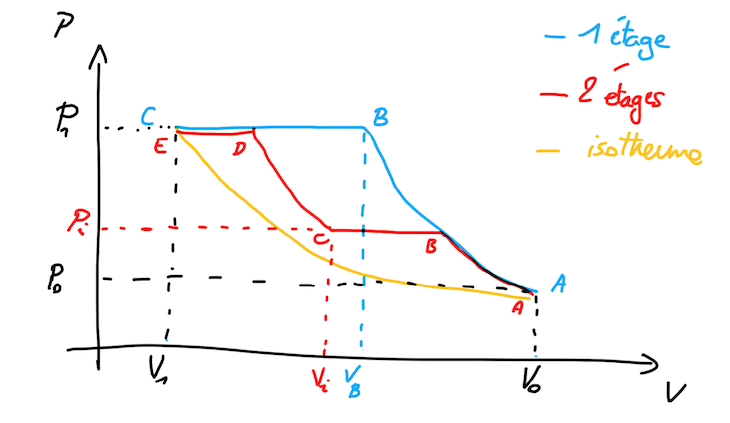
\includegraphics[width=0.5\linewidth]{thermo_cor_compresseur.png}


\item Le travail de $A\rightarrow B$ est $\frac{nR}{\gamma-1}(T_B-T_0)=\frac{(P_1V_B-P_0V_0)}{\gamma-1}$, et celui de $B\rightarrow C$ est $-P_1(V_1-V_B)$. En utilisant la loi de Laplace, on a $V_B=V_0(P_0/P_1)^{1/\gamma}$. Le travail total est donc :
\begin{align*}
	W=\frac{\gamma P_0V_0}{\gamma-1}\left(a^{\frac{\gamma-1}{\gamma}}-1 \right) 
\end{align*}

\item On a $\Delta S=\frac{nR\gamma}{\gamma-1}\ln\left( \frac{T_0}{T_1}\right)$, car transformation isentropique sur $AB$ et isobare sur $BC$. L'entropie échangée se fait à la température extérieure $T_0$, elle s'écrit :
\begin{align*}
	s_e &= \frac{Q}{T_0} \\
	&=\frac{nR\gamma}{\gamma-1}\frac{T_0-T_1}{T_0}
\end{align*}
car $Q=\frac{nR\gamma}{\gamma-1}(T_0-T_1)$ sur $BC$. 
L'entropie créée est donc :
\begin{align*}
	s_c & = \Delta S - s_e \\
	&=\frac{nR\gamma}{\gamma-1}\left[\frac{T_1}{T_0}-1-\ln\left( \frac{T_1}{T_0} \right) \right] 
\end{align*}
Celle-ci est bien positive car $x-1<\ln x$. En fonction de $a$, elle s'exprime :
\begin{align*}
	s_c =\frac{nR\gamma}{\gamma-1}\left[a^\frac{\gamma-1}{\gamma}-1-\frac{\gamma-1}{\gamma}\ln\left( a \right) \right] 
\end{align*}
en utilisant que $P^{1-\gamma}T^\gamma$ est constant sur $AB$.

\end{enumerate}

\item 

\begin{enumerate}

\item Cf le diagramme à la première question.

\item On additionne les travaux effetués. Comme les transformations $ABC$ et $CDE$ sont les mêmes, on peut utiliser les mêmes expression du travail que trouvé précédemment. On obtient :
\begin{align*}
	W'=&\frac{\gamma P_0V_0}{\gamma-1}\left[\left( \frac{P_i}{P_0}\right) ^{\frac{\gamma-1}{\gamma}}-1 \right] +\frac{\gamma P_iV_i}{\gamma-1}\left[\left( \frac{P_1}{P_i}\right) ^{\frac{\gamma-1}{\gamma}}-1 \right] \\
	=&\frac{\gamma P_0V_0}{\gamma-1}\left[\left( \frac{P_i}{P_0}\right) ^{\frac{\gamma-1}{\gamma}}+\left( \frac{P_1}{P_i}\right) ^{\frac{\gamma-1}{\gamma}}-2 \right] 
\end{align*}
\item On calcule $dW'/dP_i=0$. Aorès des calculs plus ou moins laborieux, on trouve $P_i=\sqrt{P_0P_1}$. Le travail s'exprime alors :
\begin{align*}
	W'=\frac{2\gamma P_0V_0}{\gamma-1}\left(a^{\frac{\gamma-1}{2\gamma}}-1 \right) 
\end{align*}
En posant $x=a^{\frac{\gamma-1}{2\gamma}}$, on a :
\begin{align*}
 W-W'=&\frac{\gamma P_0V_0}{\gamma-1}\left(x^2-1-2(x-1) \right) \\
 =&\frac{\gamma P_0V_0}{\gamma-1}(x^2-2x+1) \\
 =&\frac{\gamma P_0V_0}{\gamma-1}(x-1)^2\\
 &>0 
\end{align*}
Le travail est donc inférieur lorsque le compresseur a deux étages.
 
\item Avec un calcul similaire à celui du travail (il y a le log en plus), on trouve :
\begin{align*}
		s_c =\frac{2nR\gamma}{\gamma-1}\left[a^\frac{\gamma-1}{2\gamma}-1-\frac{\gamma-1}{2\gamma}\ln\left( a \right) \right] 
\end{align*}
Pour montrer que l'entropie créee est alors inférieur à la précédente, même raisonnement que la question précédente, en posant $x=a^{\frac{\gamma-1}{2\gamma}}$ :
\begin{align*}
	s_c'-s_c&=\frac{nR\gamma}{\gamma-1}\left(x^2-1-2(x-1) \right) \\
	=&\frac{\gamma nR}{\gamma-1}(x-1)^2\\
 &>0 
\end{align*}

\end{enumerate}

\item Comme on souhaite augmenter la pression tout en finissant à la même température, on peut imaginer vers cela avec une isotherme. Un diagramme de Claperon permet rapidement de voir que la travail à fournir est plus faible que les transformrations précédentes. Difficile à réaliser en pratique car une compression adiabatique réversible est beaucoup plus rapide qu'une thermalisation isotherme.

L'entropie créée dans ce cas-là est nulle, car l'entropie échangée est égale à la variation d'entropie.

\end{enumerate}

\end{correction}

\newpage

\section{Puissance d'une arme à feu $\bullet\bullet\bullet\bullet$}

On considère le canon d'une arme à feu, constitué d'un tube de diamètre $d$ et de longueur $L$, dans peut glisser sans frottement une balle (le projectile). Au coup de feu, la poudre contenue dans le volume $Sx_0$ (en pointillé) explose et dégage instantanément une énergie $Q$. La balle, de masse $m$, initialement emboitée sur la cartouche en $x_0$, est alors propulsée dans le canon, dont les parois sont supposées adiabatiques.

\begin{figure}[h!]
\centering
  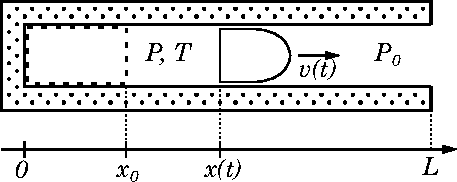
\includegraphics[width=0.65\textwidth]{thermo_fusil.pdf}
\end{figure}

On pourra modéliser le mélange d'air et de gaz issu de la combustion comme un gaz parfait de coefficient $\gamma$, à la pression $P$ et à la température $T$ lorsque le projectile est à l'abscisse $x$. Pour le calibre 5.56 OTAN, on donne : $Q\approx5000$ J, $x_0$=110 mm et $d=5,56$ mm.

\begin{enumerate}

	\item Estimer la pression $P_1$ juste après la combustion et montrer que pour des valeurs raisonnable de $L$, la pression atmosphérique $P_0$ est toujours négligeable devant $P$.
	
	\item Montrer que la vitesse de la balle en sortie de canon s'écrit :
	\begin{align*}
		v_m=\sqrt{\frac{2Q}{m}}\sqrt{1-\left(\frac{L}{x_0} \right)^{1-\gamma}}
	\end{align*}
	
	\item Calculer la pression $P_m$ et la température $T_m$ du gaz lorsque la balle sort du canon. Commenter.

\end{enumerate}